% questions.tex —— 2012 年·全国新课标卷·文科 · 题目内容片段（无答案）
% 由 tools/generate_projects.py 依来源总账自 2012/2012_数学真题_全国新课标文_试题.md 生成，勿手改（改源 MD 后重跑）


\gkpart{数学}

\begin{gknotice}
\textbf{来源说明}：本题面依据固定源 PDF 的两页 A3 题面逐题转录。PDF 第 1 页对应原卷印刷页 757，含选择题 1–12、填空题 13–16 和解答题 17–18；PDF 第 2 页对应原卷印刷页 758，含解答题 19–24。

\textbf{解析归属}：固定源不附答案或解析；配套答案与解析均由本库按本题面独立复算。

\textbf{图形说明}：第 6、7、22 题的流程图、三视图和几何图由项目内 TikZ 矢量源重绘。下列 Markdown 使用逻辑 PNG 标记供后续生成器映射，仓库不保存 PNG/JPEG/SVG 图像。
\end{gknotice}

\gkpart{一、选择题}

\begin{question}
\gkti{1}已知集合 $A=\{x\mid x^2-x-2<0\}$，$B=\{x\mid -1<x<1\}$，则\mbox{（　　）}

\begin{gkopts}(2)
\task （A）$A\subsetneqq B$
\task （B）$B\subsetneqq A$
\task （C）$A=B$
\task （D）$A\cap B=\varnothing$
\end{gkopts}

\end{question}
\begin{question}
\gkti{2}复数 $z=\dfrac{-3+i}{2+i}$ 的共轭复数是\mbox{（　　）}

\begin{gkopts}(4)
\task （A）$2+i$
\task （B）$2-i$
\task （C）$-1+i$
\task （D）$-1-i$
\end{gkopts}

\end{question}
\begin{question}
\gkti{3}在一组样本数据 $(x_1,y_1),(x_2,y_2),\cdots,(x_n,y_n)$（$n\geqslant2$，$x_1,x_2,\cdots,x_n$ 不全相等）的散点图中，若所有样本点 $(x_i,y_i)$（$i=1,2,\cdots,n$）都在直线 $y=\dfrac12x+1$ 上，则这组样本数据的样本相关系数为\mbox{（　　）}

\begin{gkopts}(4)
\task （A）$-1$
\task （B）$0$
\task （C）$\dfrac12$
\task （D）$1$
\end{gkopts}

\end{question}
\begin{question}
\gkti{4}设 $F_1,F_2$ 是椭圆 $E:\dfrac{x^2}{a^2}+\dfrac{y^2}{b^2}=1$（$a>b>0$）的左、右焦点，$P$ 为直线 $x=\dfrac{3a}{2}$ 上一点，$\triangle F_2PF_1$ 是底角为 $30^\circ$ 的等腰三角形，则 $E$ 的离心率为\mbox{（　　）}

\begin{gkopts}(4)
\task （A）$\dfrac12$
\task （B）$\dfrac23$
\task （C）$\dfrac34$
\task （D）$\dfrac45$
\end{gkopts}

\end{question}
\begin{question}
\gkti{5}已知正三角形 $ABC$ 的顶点 $A(1,1)$，$B(1,3)$，顶点 $C$ 在第一象限，若点 $(x,y)$ 在 $\triangle ABC$ 内部，则 $z=-x+y$ 的取值范围是\mbox{（　　）}

\begin{gkopts}(4)
\task （A）$(1-\sqrt3,2)$
\task （B）$(0,2)$
\task （C）$(\sqrt3-1,2)$
\task （D）$(0,1+\sqrt3)$
\end{gkopts}

\Needspace{0.4\textheight}
\end{question}
\begin{question}
\gkti{6}如果执行下面的程序框图，输入正整数 $N$（$N\geqslant2$）和实数 $a_1,a_2,\cdots,a_N$，输出 $A,B$，则\mbox{（　　）}
\nopagebreak[4]
\begin{center}\begin{tikzpicture}[
  >=stealth,
  node distance=7mm and 12mm,
  every node/.style={font=\small},
  scale=.78,
  transform shape
]
\node[draw,rounded corners,minimum width=18mm,minimum height=7mm] (start) {开始};
\node[draw,trapezium,trapezium left angle=75,trapezium right angle=105,
      minimum width=43mm,minimum height=7mm,below=of start]
      (input) {输入 $N,a_1,a_2,\ldots,a_N$};
\node[draw,minimum width=38mm,minimum height=7mm,below=of input]
      (init) {$k=1,\ A=a_1,\ B=a_1$};
\node[draw,minimum width=20mm,minimum height=7mm,below=of init]
      (read) {$x=a_k$};
\node[draw,diamond,aspect=2.2,below=of read,minimum width=25mm,minimum height=8mm]
      (max) {$x>A$};
\node[draw,minimum width=18mm,minimum height=7mm,right=of max]
      (setmax) {$A=x$};
\node[draw,diamond,aspect=2.2,below=of max,minimum width=25mm,minimum height=8mm]
      (min) {$x<B$};
\node[draw,minimum width=18mm,minimum height=7mm,left=of min]
      (setmin) {$B=x$};
\node[draw,diamond,aspect=2.2,below=of min,minimum width=25mm,minimum height=8mm]
      (done) {$k\geqslant N$};
\node[draw,minimum width=25mm,minimum height=7mm,right=of done]
      (inc) {$k=k+1$};
\node[draw,trapezium,trapezium left angle=75,trapezium right angle=105,
      minimum width=25mm,minimum height=7mm,below=of done]
      (out) {输出 $A,B$};
\node[draw,rounded corners,minimum width=18mm,minimum height=7mm,below=of out]
      (end) {结束};

\draw[->] (start)--(input)--(init)--(read)--(max);
\draw[->] (max)--node[above]{是}(setmax)--++(0,-.65) |- (done);
\draw[->] (max)--node[right]{否}(min);
\draw[->] (min)--node[above]{是}(setmin)--++(0,-.65) |- (done);
\draw[->] (min)--node[right]{否}(done);
\draw[->] (done)--node[above]{否}(inc) |- (read);
\draw[->] (done)--node[right]{是}(out)--(end);
\end{tikzpicture}
\end{center}
\nopagebreak[4]
（A）$A+B$ 为 $a_1,a_2,\cdots,a_N$ 的和　（B）$\dfrac{A+B}{2}$ 为 $a_1,a_2,\cdots,a_N$ 的算术平均数

（C）$A$ 和 $B$ 分别是 $a_1,a_2,\cdots,a_N$ 中最大的数和最小的数　（D）$A$ 和 $B$ 分别是 $a_1,a_2,\cdots,a_N$ 中最小的数和最大的数

\Needspace{0.4\textheight}
\end{question}
\begin{question}
\gkti{7}如图，网格上小正方形的边长为 $1$，粗线画出的是某几何体的三视图，则此几何体的体积为\mbox{（　　）}
\nopagebreak[4]
\begin{center}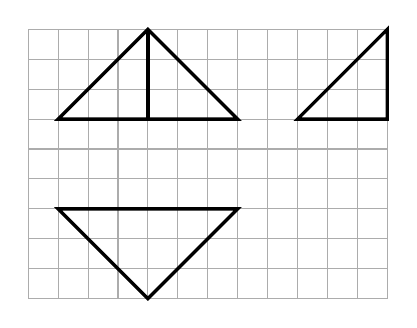
\begin{tikzpicture}[scale=.38]
  \draw[gray!65] (0,0) grid (12,9);
  \draw[very thick] (1,6)--(7,6)--(4,9)--cycle;
  \draw[very thick] (4,6)--(4,9);
  \draw[very thick] (9,6)--(12,6)--(12,9)--cycle;
  \draw[very thick] (1,3)--(7,3)--(4,0)--cycle;
\end{tikzpicture}
\end{center}
\nopagebreak[4]
\begin{gkopts}(4)
\task （A）$6$
\task （B）$9$
\task （C）$12$
\task （D）$18$
\end{gkopts}

\end{question}
\begin{question}
\gkti{8}平面 $\alpha$ 截球 $O$ 的球面所得圆的半径为 $1$，球心 $O$ 到平面 $\alpha$ 的距离为 $\sqrt2$，则此球的体积为\mbox{（　　）}

\begin{gkopts}(4)
\task （A）$\sqrt6\pi$
\task （B）$4\sqrt3\pi$
\task （C）$4\sqrt6\pi$
\task （D）$6\sqrt3\pi$
\end{gkopts}

\end{question}
\begin{question}
\gkti{9}已知 $\omega>0$，$0<\varphi<\pi$，直线 $x=\dfrac\pi4$ 和 $x=\dfrac{5\pi}4$ 是函数 $f(x)=\sin(\omega x+\varphi)$ 图象的两条相邻的对称轴，则 $\varphi=$\mbox{（　　）}

\begin{gkopts}(2)
\task （A）$\dfrac\pi4$
\task （B）$\dfrac\pi3$
\task （C）$\dfrac\pi2$
\task （D）$\dfrac{3\pi}4$
\end{gkopts}

\end{question}
\begin{question}
\gkti{10}等轴双曲线 $C$ 的中心在原点，焦点在 $x$ 轴上，$C$ 与抛物线 $y^2=16x$ 的准线交于 $A,B$ 两点，$|AB|=4\sqrt3$，则 $C$ 的实轴长为\mbox{（　　）}

\begin{gkopts}(4)
\task （A）$\sqrt2$
\task （B）$2\sqrt2$
\task （C）$4$
\task （D）$8$
\end{gkopts}

\end{question}
\begin{question}
\gkti{11}当 $0<x\leqslant\dfrac12$ 时，$4^x<\log_a x$，则 $a$ 的取值范围是\mbox{（　　）}

\begin{gkopts}(2)
\task （A）$\left(0,\dfrac{\sqrt2}{2}\right)$
\task （B）$\left(\dfrac{\sqrt2}{2},1\right)$
\task （C）$(1,\sqrt2)$
\task （D）$(\sqrt2,2)$
\end{gkopts}

\end{question}
\begin{question}
\gkti{12}数列 $\{a_n\}$ 满足 $a_{n+1}+(-1)^n a_n=2n-1$，则 $\{a_n\}$ 的前 $60$ 项和为\mbox{（　　）}

\begin{gkopts}(4)
\task （A）$3690$
\task （B）$3660$
\task （C）$1845$
\task （D）$1830$
\end{gkopts}

\end{question}
\gkpart{二、填空题}

\begin{question}
\gkti{13}曲线 $y=x(3\ln x+1)$ 在点 $(1,1)$ 处的切线方程为\gkblank{}。

\end{question}
\begin{question}
\gkti{14}等比数列 $\{a_n\}$ 的前 $n$ 项和为 $S_n$，若 $S_3+3S_2=0$，则公比 $q=$\gkblank{}。

\end{question}
\begin{question}
\gkti{15}已知向量 $\boldsymbol a,\boldsymbol b$ 夹角为 $45^\circ$，且 $|\boldsymbol a|=1$，$|2\boldsymbol a-\boldsymbol b|=\sqrt{10}$，则 $|\boldsymbol b|=$\gkblank{}。

\end{question}
\begin{question}
\gkti{16}设函数 $f(x)=\dfrac{(x+1)^2+\sin x}{x^2+1}$ 的最大值为 $M$，最小值为 $m$，则 $M+m=$\gkblank{}。

\end{question}
\gkpart{三、解答题}

\begin{question}
\gkti{17}已知 $a,b,c$ 分别为 $\triangle ABC$ 三个内角 $A,B,C$ 的对边，$a\cos C+\sqrt3a\sin C-b-c=0$。

（1）　求 $A$；

（2）　若 $a=2$，$\triangle ABC$ 的面积为 $\sqrt3$，求 $b,c$。

\end{question}
\begin{question}
\gkti{18}某花店每天以每枝 $5$ 元的价格从农场购进若干枝玫瑰花，然后以每枝 $10$ 元的价格出售，如果当天卖不完，剩下的玫瑰花作垃圾处理。

（1）　若花店一天购进 $16$ 枝玫瑰花，求当天的利润 $y$（单位：元）关于当天需求量 $n$（单位：枝，$n\in\mathbb N$）的函数解析式；

（2）　花店记录了 $100$ 天玫瑰花的日需求量（单位：枝），整理得下表：

\begin{center}
\begingroup\setlength{\tabcolsep}{4pt}
\begin{tabular}{lrrrrrrr}
\toprule
日需求量 $n$ & 14 & 15 & 16 & 17 & 18 & 19 & 20 \\
\midrule
频数 & 10 & 20 & 16 & 16 & 15 & 13 & 10 \\
\bottomrule
\end{tabular}
\endgroup
\end{center}

以 $100$ 天记录的各需求量的频率作为各需求量发生的概率。

① 假设花店在这 $100$ 天内每天购进 $17$ 枝玫瑰花，求这 $100$ 天的日利润（单位：元）的平均数；

② 若花店一天购进 $17$ 枝玫瑰花，以 $100$ 天记录的各需求量的频率作为各需求量发生的概率，求当天的利润不少于 $75$ 元的概率。

\end{question}
\begin{question}
\gkti{19}如图，三棱柱 $ABC-A_1B_1C_1$ 中，侧棱垂直底面，$\angle ACB=90^\circ$，$AC=BC=\dfrac12AA_1$，$D$ 是棱 $AA_1$ 的中点。

（1）　证明：平面 $BDC_1\perp$ 平面 $BDC$；

（2）　平面 $BDC_1$ 分此棱柱为两部分，求这两部分体积的比。

\end{question}
\begin{question}
\gkti{20}设抛物线 $C:x^2=2py$（$p>0$）的焦点为 $F$，准线为 $l$，$A$ 为 $C$ 上一点，已知以 $F$ 为圆心、$FA$ 为半径的圆 $F$ 交 $l$ 于 $B,D$ 两点。

（1）　若 $\angle BFD=90^\circ$，$\triangle ABD$ 的面积为 $4\sqrt2$，求 $p$ 的值及圆 $F$ 的方程；

（2）　若 $A,B,F$ 三点在同一直线 $m$ 上，直线 $n$ 与 $m$ 平行，且 $n$ 与 $C$ 只有一个公共点，求坐标原点到 $m,n$ 距离的比值。

\end{question}
\begin{question}
\gkti{21}设函数 $f(x)=\mathrm e^x-ax-2$。

（1）　求 $f(x)$ 的单调区间；

（2）　若 $a=1$，$k$ 为整数，且当 $x>0$ 时，$(x-k)f'(x)+x+1>0$，求 $k$ 的最大值。

\Needspace{0.4\textheight}
\end{question}
\begin{question}
\gkti{22}如图，$D,E$ 分别为 $\triangle ABC$ 边 $AB,AC$ 的中点，直线 $DE$ 交 $\triangle ABC$ 的外接圆于 $F,G$ 两点。若 $CF\parallel AB$，证明：

（1）　$CD=BC$；

（2）　$\triangle BCD\sim\triangle GBD$。
\nopagebreak[4]
\begin{center}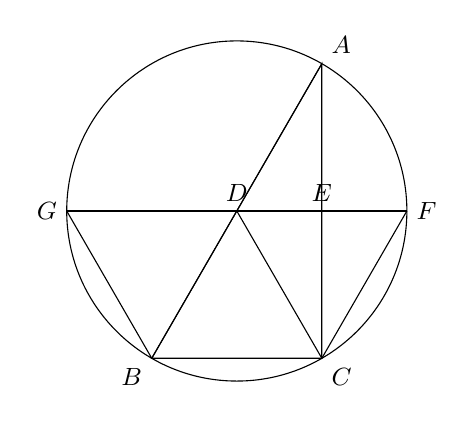
\begin{tikzpicture}[scale=.72, every node/.style={font=\small}]
  \coordinate (G) at (-3,0);
  \coordinate (F) at (3,0);
  \coordinate (A) at (1.5,2.598);
  \coordinate (B) at (-1.5,-2.598);
  \coordinate (C) at (1.5,-2.598);
  \coordinate (D) at (0,0);
  \coordinate (E) at (1.5,0);
  \draw (0,0) circle (3);
  \draw (G)--(F);
  \draw (A)--(B)--(C)--cycle;
  \draw (D)--(C);
  \draw (G)--(B);
  \draw (C)--(F);
  \draw (A)--(C);
  \draw (A)--(B);
  \node[above right] at (A) {$A$};
  \node[below left] at (B) {$B$};
  \node[below right] at (C) {$C$};
  \node[above] at (D) {$D$};
  \node[above] at (E) {$E$};
  \node[left] at (G) {$G$};
  \node[right] at (F) {$F$};
\end{tikzpicture}
\end{center}
\nopagebreak[4]
\end{question}
\begin{question}
\gkti{23}已知曲线 $C_1$ 的参数方程是 $\begin{cases}x=2\cos\varphi,\\y=3\sin\varphi,\end{cases}$（$\varphi$ 是参数）．以坐标原点为极点，$x$ 轴的非负半轴为极轴建立极坐标系，曲线 $C_2$ 的极坐标方程是 $\rho=2$，正方形 $ABCD$ 的顶点都在 $C_2$ 上，且 $A,B,C,D$ 依逆时针次序排列，点 $A$ 的极坐标为 $(2,\dfrac\pi3)$。

（1）　求点 $A,B,C,D$ 的直角坐标；

（2）　设 $P$ 为 $C_1$ 上任意一点，求 $|PA|^2+|PB|^2+|PC|^2+|PD|^2$ 的取值范围。

\end{question}
\begin{question}
\gkti{24}已知函数 $f(x)=|x+a|+|x-2|$。

（1）　当 $a=-3$ 时，求不等式 $f(x)\geqslant3$ 的解集；

（2）　若 $f(x)\leqslant|x-4|$ 的解集包含 $[1,2]$，求 $a$ 的取值范围。

\end{question}